% Auto-generated by experiments.analysis.generate_win_counts --- do not edit.
\begin{figure}[H]
\centering
\adjustbox{max width=\textwidth}{%
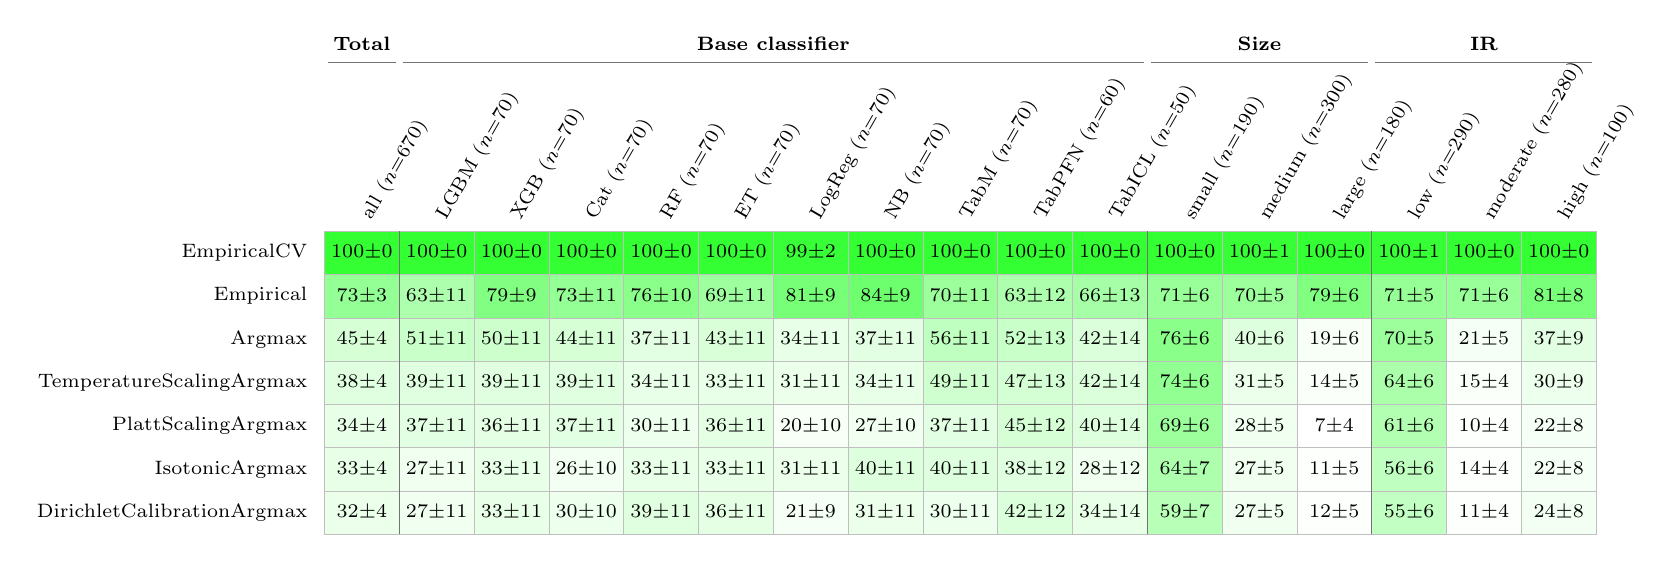
\begin{tikzpicture}[
    x=0.95cm, y=0.55cm,
    cell/.style={rectangle, draw=black!25, line width=0.2pt,
        minimum width=0.95cm, minimum height=0.55cm,
        anchor=center, font=\scriptsize, inner sep=0pt},
    rowlbl/.style={font=\scriptsize, anchor=east},
    collbl/.style={font=\scriptsize, anchor=west, rotate=60},
    grouplbl/.style={font=\scriptsize\bfseries, anchor=south},
    sep/.style={draw=black!55, line width=0.5pt},
]
\node[cell, fill=green!80] at (1, 7) {$100{\pm}0$};
\node[cell, fill=green!80] at (2, 7) {$100{\pm}0$};
\node[cell, fill=green!80] at (3, 7) {$100{\pm}0$};
\node[cell, fill=green!80] at (4, 7) {$100{\pm}0$};
\node[cell, fill=green!80] at (5, 7) {$100{\pm}0$};
\node[cell, fill=green!80] at (6, 7) {$100{\pm}0$};
\node[cell, fill=green!78] at (7, 7) {$99{\pm}2$};
\node[cell, fill=green!80] at (8, 7) {$100{\pm}0$};
\node[cell, fill=green!80] at (9, 7) {$100{\pm}0$};
\node[cell, fill=green!80] at (10, 7) {$100{\pm}0$};
\node[cell, fill=green!80] at (11, 7) {$100{\pm}0$};
\node[cell, fill=green!80] at (12, 7) {$100{\pm}0$};
\node[cell, fill=green!79] at (13, 7) {$100{\pm}1$};
\node[cell, fill=green!80] at (14, 7) {$100{\pm}0$};
\node[cell, fill=green!79] at (15, 7) {$100{\pm}1$};
\node[cell, fill=green!80] at (16, 7) {$100{\pm}0$};
\node[cell, fill=green!80] at (17, 7) {$100{\pm}0$};
\node[cell, fill=green!42] at (1, 6) {$73{\pm}3$};
\node[cell, fill=green!32] at (2, 6) {$63{\pm}11$};
\node[cell, fill=green!49] at (3, 6) {$79{\pm}9$};
\node[cell, fill=green!42] at (4, 6) {$73{\pm}11$};
\node[cell, fill=green!46] at (5, 6) {$76{\pm}10$};
\node[cell, fill=green!38] at (6, 6) {$69{\pm}11$};
\node[cell, fill=green!53] at (7, 6) {$81{\pm}9$};
\node[cell, fill=green!57] at (8, 6) {$84{\pm}9$};
\node[cell, fill=green!39] at (9, 6) {$70{\pm}11$};
\node[cell, fill=green!32] at (10, 6) {$63{\pm}12$};
\node[cell, fill=green!35] at (11, 6) {$66{\pm}13$};
\node[cell, fill=green!40] at (12, 6) {$71{\pm}6$};
\node[cell, fill=green!39] at (13, 6) {$70{\pm}5$};
\node[cell, fill=green!50] at (14, 6) {$79{\pm}6$};
\node[cell, fill=green!41] at (15, 6) {$71{\pm}5$};
\node[cell, fill=green!40] at (16, 6) {$71{\pm}6$};
\node[cell, fill=green!52] at (17, 6) {$81{\pm}8$};
\node[cell, fill=green!16] at (1, 5) {$45{\pm}4$};
\node[cell, fill=green!21] at (2, 5) {$51{\pm}11$};
\node[cell, fill=green!20] at (3, 5) {$50{\pm}11$};
\node[cell, fill=green!16] at (4, 5) {$44{\pm}11$};
\node[cell, fill=green!11] at (5, 5) {$37{\pm}11$};
\node[cell, fill=green!15] at (6, 5) {$43{\pm}11$};
\node[cell, fill=green!9] at (7, 5) {$34{\pm}11$};
\node[cell, fill=green!11] at (8, 5) {$37{\pm}11$};
\node[cell, fill=green!25] at (9, 5) {$56{\pm}11$};
\node[cell, fill=green!21] at (10, 5) {$52{\pm}13$};
\node[cell, fill=green!14] at (11, 5) {$42{\pm}14$};
\node[cell, fill=green!46] at (12, 5) {$76{\pm}6$};
\node[cell, fill=green!13] at (13, 5) {$40{\pm}6$};
\node[cell, fill=green!3] at (14, 5) {$19{\pm}6$};
\node[cell, fill=green!39] at (15, 5) {$70{\pm}5$};
\node[cell, fill=green!4] at (16, 5) {$21{\pm}5$};
\node[cell, fill=green!11] at (17, 5) {$37{\pm}9$};
\node[cell, fill=green!12] at (1, 4) {$38{\pm}4$};
\node[cell, fill=green!12] at (2, 4) {$39{\pm}11$};
\node[cell, fill=green!12] at (3, 4) {$39{\pm}11$};
\node[cell, fill=green!12] at (4, 4) {$39{\pm}11$};
\node[cell, fill=green!9] at (5, 4) {$34{\pm}11$};
\node[cell, fill=green!9] at (6, 4) {$33{\pm}11$};
\node[cell, fill=green!8] at (7, 4) {$31{\pm}11$};
\node[cell, fill=green!9] at (8, 4) {$34{\pm}11$};
\node[cell, fill=green!19] at (9, 4) {$49{\pm}11$};
\node[cell, fill=green!17] at (10, 4) {$47{\pm}13$};
\node[cell, fill=green!14] at (11, 4) {$42{\pm}14$};
\node[cell, fill=green!43] at (12, 4) {$74{\pm}6$};
\node[cell, fill=green!8] at (13, 4) {$31{\pm}5$};
\node[cell, fill=green!2] at (14, 4) {$14{\pm}5$};
\node[cell, fill=green!33] at (15, 4) {$64{\pm}6$};
\node[cell, fill=green!2] at (16, 4) {$15{\pm}4$};
\node[cell, fill=green!7] at (17, 4) {$30{\pm}9$};
\node[cell, fill=green!9] at (1, 3) {$34{\pm}4$};
\node[cell, fill=green!11] at (2, 3) {$37{\pm}11$};
\node[cell, fill=green!10] at (3, 3) {$36{\pm}11$};
\node[cell, fill=green!11] at (4, 3) {$37{\pm}11$};
\node[cell, fill=green!7] at (5, 3) {$30{\pm}11$};
\node[cell, fill=green!10] at (6, 3) {$36{\pm}11$};
\node[cell, fill=green!3] at (7, 3) {$20{\pm}10$};
\node[cell, fill=green!6] at (8, 3) {$27{\pm}10$};
\node[cell, fill=green!11] at (9, 3) {$37{\pm}11$};
\node[cell, fill=green!16] at (10, 3) {$45{\pm}12$};
\node[cell, fill=green!13] at (11, 3) {$40{\pm}14$};
\node[cell, fill=green!39] at (12, 3) {$69{\pm}6$};
\node[cell, fill=green!6] at (13, 3) {$28{\pm}5$};
\node[cell, fill=green!0] at (14, 3) {$7{\pm}4$};
\node[cell, fill=green!30] at (15, 3) {$61{\pm}6$};
\node[cell, fill=green!1] at (16, 3) {$10{\pm}4$};
\node[cell, fill=green!4] at (17, 3) {$22{\pm}8$};
\node[cell, fill=green!9] at (1, 2) {$33{\pm}4$};
\node[cell, fill=green!6] at (2, 2) {$27{\pm}11$};
\node[cell, fill=green!9] at (3, 2) {$33{\pm}11$};
\node[cell, fill=green!5] at (4, 2) {$26{\pm}10$};
\node[cell, fill=green!9] at (5, 2) {$33{\pm}11$};
\node[cell, fill=green!9] at (6, 2) {$33{\pm}11$};
\node[cell, fill=green!8] at (7, 2) {$31{\pm}11$};
\node[cell, fill=green!13] at (8, 2) {$40{\pm}11$};
\node[cell, fill=green!13] at (9, 2) {$40{\pm}11$};
\node[cell, fill=green!12] at (10, 2) {$38{\pm}12$};
\node[cell, fill=green!6] at (11, 2) {$28{\pm}12$};
\node[cell, fill=green!32] at (12, 2) {$64{\pm}7$};
\node[cell, fill=green!6] at (13, 2) {$27{\pm}5$};
\node[cell, fill=green!1] at (14, 2) {$11{\pm}5$};
\node[cell, fill=green!25] at (15, 2) {$56{\pm}6$};
\node[cell, fill=green!1] at (16, 2) {$14{\pm}4$};
\node[cell, fill=green!4] at (17, 2) {$22{\pm}8$};
\node[cell, fill=green!8] at (1, 1) {$32{\pm}4$};
\node[cell, fill=green!6] at (2, 1) {$27{\pm}11$};
\node[cell, fill=green!9] at (3, 1) {$33{\pm}11$};
\node[cell, fill=green!7] at (4, 1) {$30{\pm}10$};
\node[cell, fill=green!12] at (5, 1) {$39{\pm}11$};
\node[cell, fill=green!10] at (6, 1) {$36{\pm}11$};
\node[cell, fill=green!4] at (7, 1) {$21{\pm}9$};
\node[cell, fill=green!8] at (8, 1) {$31{\pm}11$};
\node[cell, fill=green!7] at (9, 1) {$30{\pm}11$};
\node[cell, fill=green!14] at (10, 1) {$42{\pm}12$};
\node[cell, fill=green!9] at (11, 1) {$34{\pm}14$};
\node[cell, fill=green!28] at (12, 1) {$59{\pm}7$};
\node[cell, fill=green!6] at (13, 1) {$27{\pm}5$};
\node[cell, fill=green!1] at (14, 1) {$12{\pm}5$};
\node[cell, fill=green!24] at (15, 1) {$55{\pm}6$};
\node[cell, fill=green!1] at (16, 1) {$11{\pm}4$};
\node[cell, fill=green!5] at (17, 1) {$24{\pm}8$};
\node[rowlbl] at (0.4, 7) {EmpiricalCV};
\node[rowlbl] at (0.4, 6) {Empirical};
\node[rowlbl] at (0.4, 5) {Argmax};
\node[rowlbl] at (0.4, 4) {TemperatureScalingArgmax};
\node[rowlbl] at (0.4, 3) {PlattScalingArgmax};
\node[rowlbl] at (0.4, 2) {IsotonicArgmax};
\node[rowlbl] at (0.4, 1) {DirichletCalibrationArgmax};
\node[collbl] at (1, 7.6) {all ($n{=}670$)};
\node[collbl] at (2, 7.6) {LGBM ($n{=}70$)};
\node[collbl] at (3, 7.6) {XGB ($n{=}70$)};
\node[collbl] at (4, 7.6) {Cat ($n{=}70$)};
\node[collbl] at (5, 7.6) {RF ($n{=}70$)};
\node[collbl] at (6, 7.6) {ET ($n{=}70$)};
\node[collbl] at (7, 7.6) {LogReg ($n{=}70$)};
\node[collbl] at (8, 7.6) {NB ($n{=}70$)};
\node[collbl] at (9, 7.6) {TabM ($n{=}70$)};
\node[collbl] at (10, 7.6) {TabPFN ($n{=}60$)};
\node[collbl] at (11, 7.6) {TabICL ($n{=}50$)};
\node[collbl] at (12, 7.6) {small ($n{=}190$)};
\node[collbl] at (13, 7.6) {medium ($n{=}300$)};
\node[collbl] at (14, 7.6) {large ($n{=}180$)};
\node[collbl] at (15, 7.6) {low ($n{=}290$)};
\node[collbl] at (16, 7.6) {moderate ($n{=}280$)};
\node[collbl] at (17, 7.6) {high ($n{=}100$)};
\draw[black!55, line width=0.5pt] (0.55, 11.4) -- (1.45, 11.4);
\node[grouplbl] at (1.0, 11.450000000000001) {Total};
\draw[black!55, line width=0.5pt] (1.55, 11.4) -- (11.45, 11.4);
\node[grouplbl] at (6.5, 11.450000000000001) {Base classifier};
\draw[black!55, line width=0.5pt] (11.55, 11.4) -- (14.45, 11.4);
\node[grouplbl] at (13.0, 11.450000000000001) {Size};
\draw[black!55, line width=0.5pt] (14.55, 11.4) -- (17.45, 11.4);
\node[grouplbl] at (16.0, 11.450000000000001) {IR};
\draw[sep] (1.5, 0.5) -- (1.5, 7.5);
\draw[sep] (11.5, 0.5) -- (11.5, 7.5);
\draw[sep] (14.5, 0.5) -- (14.5, 7.5);
\end{tikzpicture}%
}
\caption{Per-strategy win/tie rates on binary maximization metrics. Each cell reads ``$r{\pm}H$'': $r$ is the percentage of (dataset, model, objective) cells in the slice where the strategy won or tied the per-row best under the $\pm 1$ SE overlap rule, and $H$ is the half-width of a 95\% cluster-bootstrap confidence interval for $r$ (percentage points). Shading is a quadratic ($\mathrm{rate}^2$) scale of $r$. Strategies are sorted by overall win rate; ``$n$'' under each column header is the maximum applicable cell count for that slice.}%
\label{fig:win-counts-binary-max}
\end{figure}
